\documentclass[letterpaper,12pt]{article}

% --- Packages
%\usepackage[paperwidth=5.5in, paperheight=4.25in,margin=0in]{geometry}

\usepackage{tikz} 			%draw

\usepackage{fontspec}		%Set font
\setmainfont{Orbit}         % special by Evan Pittson Design

% --- Formatting
\pagenumbering{gobble}


% --- Defined Values
%% Variables
\newcommand{\altMargin}{1}
\newcommand{\cardHeight}{4.25}%{\paperheight-\altMargin}
\newcommand{\cardWidth}{5.5}%{\paperwidth-\altMargin}
% Style Variables
\newcommand{\setNumber}{0}
\newcommand{\cardNumber}{1}
\newcommand{ \cardTitleSty }[1]{\raggedright \uppercase{#1}}
\newcommand{\qrkNumSty}{ 	 QRK M$7_{\setNumber} 20200530:\cardNumber-\setNumber/20$ T$9$ }
% Instructions For
\newcommand{\sender}{Sender}
\newcommand{\recipient}{Before Reading}
% Instructions
\newcommand{\single}[1]{#1}							
\newcommand{\double}[2]{#1,#2}
\newcommand{\triple}[3]{#1,#2,3}
\newcommand{\singleSingle}[2]{#1,#2}
\newcommand{\doubleSingle}[3]{#1,#2,#3}
\newcommand{\tripleSingle}[4]{#1,#2,#3,#4}
\newcommand{\singleDouble}[3]{#1,#2,#3}
\newcommand{\doubleDouble}[4]{#1,#2,#3,#4}
\newcommand{\tripleDouble}[5]{#1,#2,#3,#4,#5}
\newcommand{\singleTriple}[4]{#1,#2,#3,#4}
\newcommand{\doubleTriple}[5]{#1,#2,#3,#4,#5}
\newcommand{\tripleTriple}[6]{#1,#2,#3,#4,#5,#6}



\begin{document}

\begin{figure}
%\resizebox{5.5in}{4.25in}
%	{
	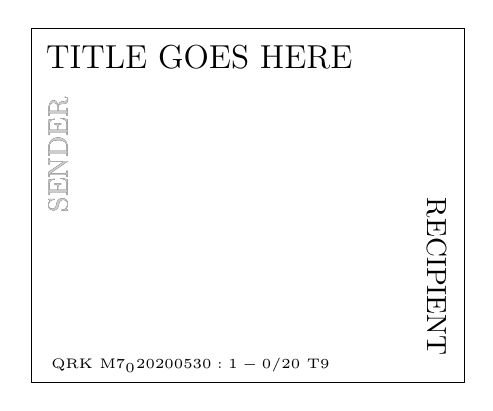
\begin{tikzpicture}[]
		
		% card
    	\draw (-2.75,-2.25) rectangle (2.75, 2.25);
    	
    	% title
    	\node[anchor=north west] at (-2.80, 2.15) {\cardTitleSty{ \large Title Goes Here}};
    	
    	% QRK Number
    	\node[anchor=south west] at (-2.70, -2.25) { \tiny \qrkNumSty};
    	
%    	% sender reflection
%    	\node[anchor=south west, rotate = -90, text = black!30!white ] at (-2.36, 1.63) {\cardTitleSty{ \normalsize Sender }};
    	% sender label  - on
    	\node[anchor=north east, rotate = 90] at (-2.65,1.5) {\cardTitleSty{ \normalsize Sender }};
    	 % sender label  - off
    	\node[anchor=north east, rotate = 90, text = black!20!white] at (-2.65,1.5) {\cardTitleSty{ \normalsize Sender }};
    	
%    	% recipient reflection 
%    	\node[anchor=south west, rotate = 90, text = black!20!white] at (2.65,-2.25) {\cardTitleSty{ \normalsize Recipient }}; % 2.345 for label if uncomment relfection

    	% recipient label - on
    	\node[anchor=north east, rotate = -90 ] at (2.645, -2.03) {\cardTitleSty{\normalsize Recipient}};
%    	% recipient label - off
%    	\node[anchor=north east, rotate = -90, text = black!20!white ] at (2.645, -2.03) {\cardTitleSty{\normalsize Recipient}};
    			
		
	\end{tikzpicture}
%	}
\end{figure}

\end{document}